\documentclass[twoside]{article}
\usepackage{amsgen,amsmath,amstext,amsbsy,amsopn,amssymb,hyperref}
\usepackage{graphicx}
\usepackage{epsfig}

\setlength{\oddsidemargin}{0.1 in} \setlength{\evensidemargin}{-0.1
in} \setlength{\topmargin}{-0.6 in} \setlength{\textwidth}{6.5 in}
\setlength{\textheight}{10.4 in} \setlength{\headsep}{0.1 in}
\setlength{\parindent}{0 in} \setlength{\parskip}{0.1 in}

\newcommand{\homework}[2]{
   \pagestyle{myheadings}
   \thispagestyle{plain}
   \newpage
   \setcounter{page}{1}
   \noindent
   \begin{center}
   \framebox{
      \vbox{\vspace{2mm}
       \hbox to 6.28in { {\bf Math 1700:~Elementary Statistics \hfill} }
       \vspace{6mm}
       \hbox to 6.28in { {\Large \hfill #1 (#2)  \hfill} }
       \vspace{6mm}
      \vspace{2mm}}
   }
   \end{center}
   \markboth{#1}{#1}
   \vspace*{4mm}
}

\newcommand{\bbF}{\mathbb{F}}
\newcommand{\bbX}{\mathbb{X}}
\newcommand{\bI}{\mathbf{I}}
\newcommand{\bX}{\mathbf{X}}
\newcommand{\bY}{\mathbf{Y}}
\newcommand{\bepsilon}{\boldsymbol{\epsilon}}
\newcommand{\balpha}{\boldsymbol{\alpha}}
\newcommand{\bbeta}{\boldsymbol{\beta}}
\newcommand{\0}{\mathbf{0}}

\begin{document}

\homework{$5^{th}$ and $6^{th}$ Weeks Summary}{10/02/25}
\vspace{-.3in}
\begin{itemize}
\item \textbf{Continuous Random Variable}: A quantitative random variable that can assume an uncountable (continuum of values).
\item The \textbf{normal distribution} is considered the single most important probability distribution.
\item All normal distributions are related to one distribution, called \textbf{standard normal distribution}.
\item Properties of the \textbf{standard normal distribution}:
\subitem The total area under the normal curve is equal to 1.
\subitem The distribution is mounded and symmetric; it extends indefinitely in both directions.
\subitem The distribution has a mean of $0$ and a standard deviation of $1$.
\subitem The mean divides the area in half, $0.50$ each side.
\subitem Nearly all the area is between $z=-3.00$ and $z=3.00$.
\item \textbf{Probability distribution}: A formula or a list that provides the probability for a continuous random variable having a value falling within a specified interval. $P(a<x<b) = \ ?$
\item The standardized value is called a \textbf{z-score}. $z=\dfrac{x-\mu}{\sigma}$
\item Finding Normal Probabilities :
\subitem Less than: $P(x<a)=P\Bigl(\dfrac{x-\mu}{\sigma}<\dfrac{a-\mu}{\sigma}\Bigr)=P(z<z_a)$
\subitem Greater than: $P(x>b)=P(z>z_b)=1-P(z<z_b)$
\subitem Between two numbers: $P(a<x<b)=P(z_a<z<z_b)=P(z<z_b)-P(z<z_a)$
\item The convention that we will use is \textbf{notation $z(\alpha)$} for a specific $z$-score, where $\alpha$ represents the \textbf{``area to the right''} of the being named.
\item The probabilities associated with a \textbf{binomial distribution} with $n$ trials and probability of success$ = p$, can be reasonably \textbf{approximated} by using the \textbf{normal probability} distribution with mean: $\mu=np$ and $\sigma^2=np(1-p)$.
\item \textbf{Rule of thumb:} normal distribution provides a reasonable approximation to a binomial probability distribution whenever the values of $np$ \ and \ $n(1-p)$ both \textbf{equal} or \textbf{exceed} $5$.
\item \href{https://www.geogebra.org/m/knAbwFo2}{Normal Approximation to Binomial Applet}
\begin{figure}[h]
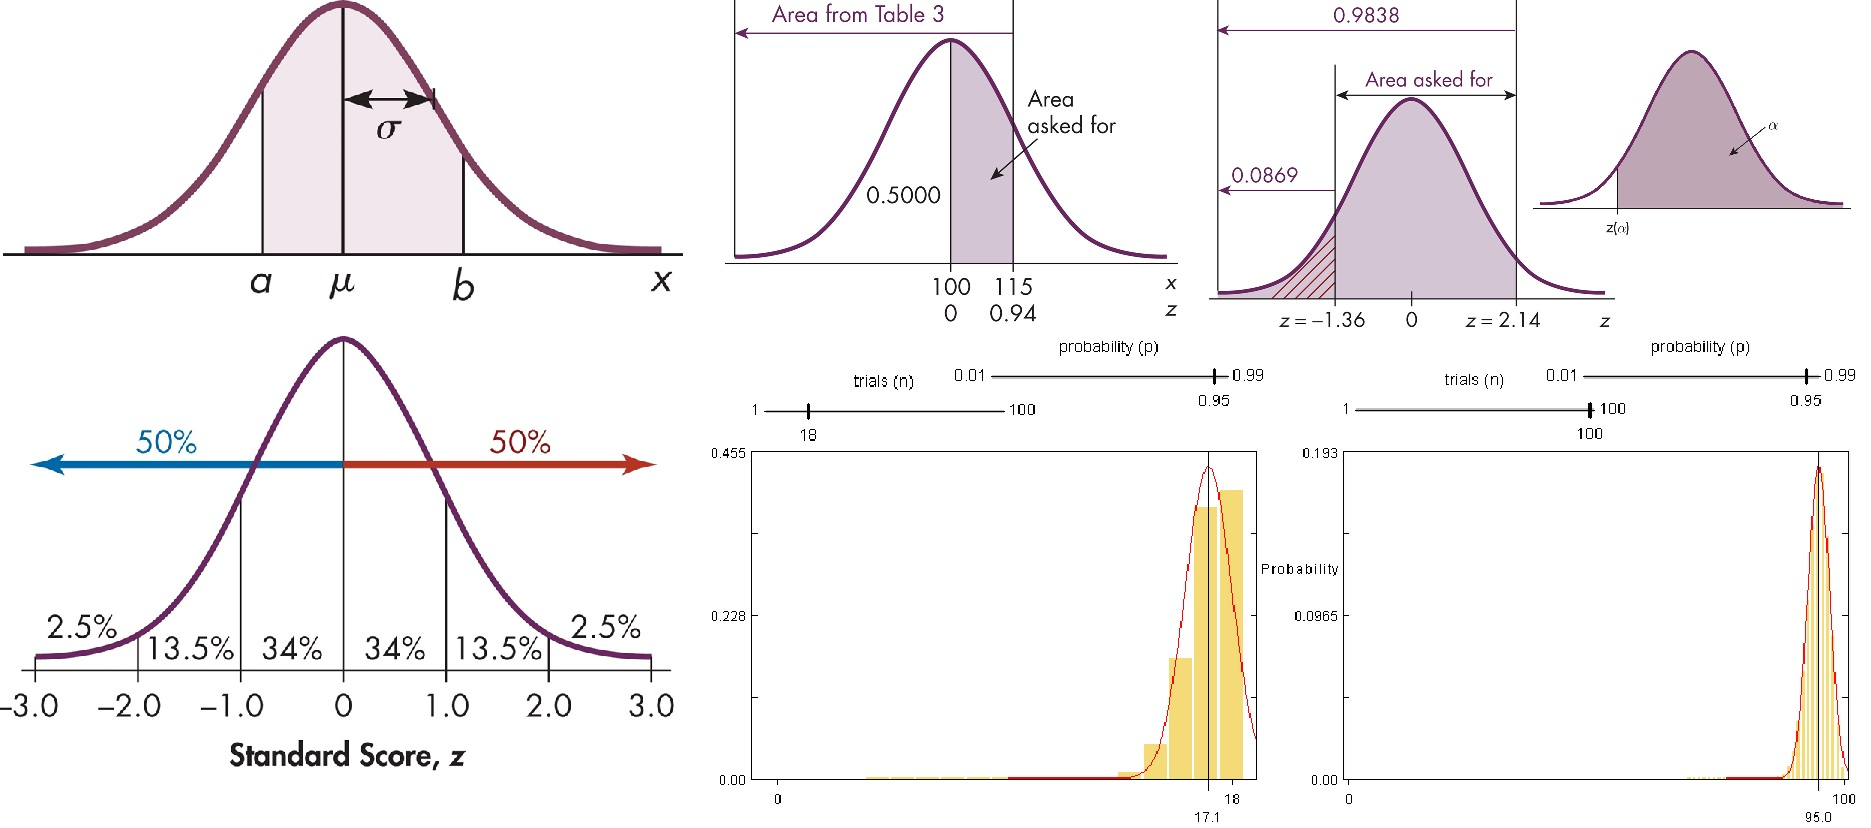
\includegraphics[angle=0,width=\textwidth] {graphs7.jpg}
\end{figure}

\item What is the relationship between distribution of $x$ and $\bar{x}$?
\begin{figure}[h]
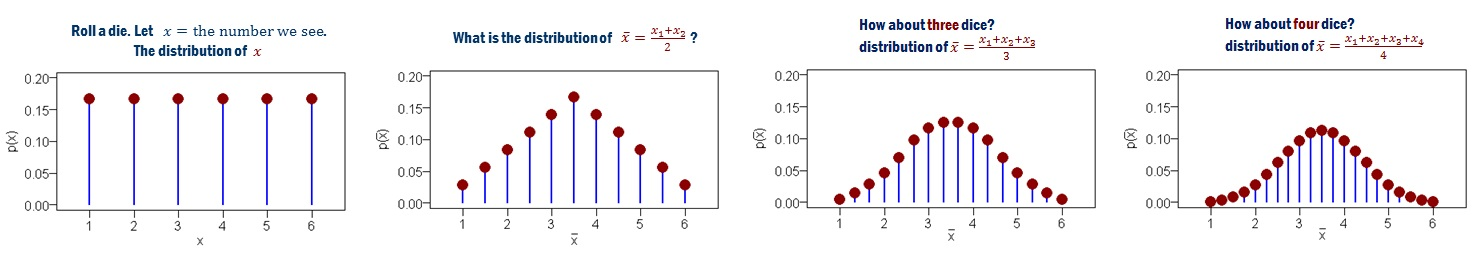
\includegraphics[angle=0,width=\textwidth] {graphs8-0.jpg}
\end{figure}
\vspace{-.1in}
\item Sampling distribution of a sample statistic
\subitem The distribution of values for a \textbf{sample statistic} obtained from repeated samples, all of \textbf{the same size} and all drawn from the same population.
\item \href{http://www.mssc.mu.edu/~mehdi/applets/sample_dist/index.html}{Sampling distribution applet}
\item Random sampling
\subitem A sample obtained in such a way that each possible sample of fixed size $n$ has an equal probability of being selected.
\item Sampling distribution of sample means (\textbf{SDSM})
\subitem $\mu_{\bar{x}}=\mu$
\subitem $\sigma^2_{\bar{x}}=\dfrac{\sigma^2}{n}$
\subitem $\sigma_{\bar{x}}=\dfrac{\sigma}{\sqrt{n}}$
\item Central limit theorem (\textbf{CLT})
\subitem The sampling distribution of sample means will more closely resemble the normal distribution as the \textbf{sample size increases}.
\item Standard error of the mean (${\sigma}/{\sqrt{n}}$):
\subitem is used to denote to the standard deviation of the sampling distribution of sample means.
\begin{figure}[h]
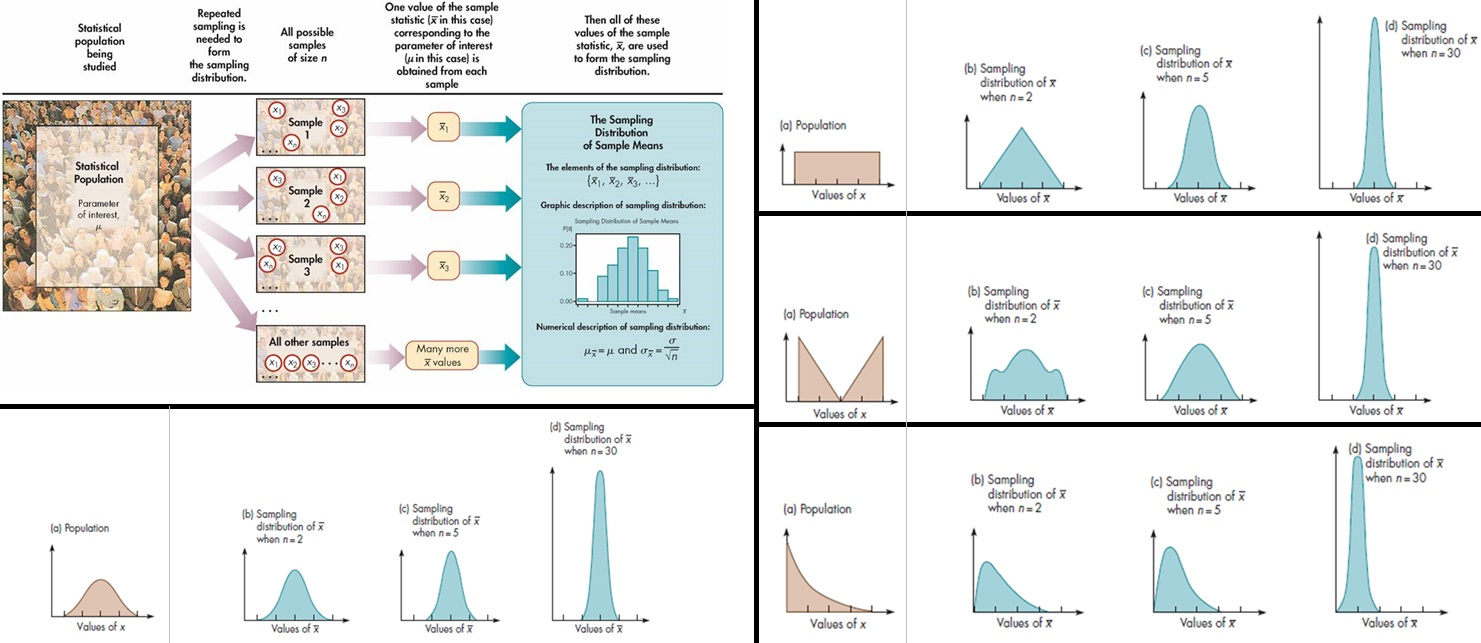
\includegraphics[angle=0,width=\textwidth] {graphs8.jpg}
\end{figure}
\end{itemize}
\end{document}
